\section{Ticks, Song Stats und Hexbefehle}

Dieses Kapitel beschäftigt sich rund um das Thema Hexwerte und Hexbefehle. Es werden die meisten, aber nicht alle Hexbefehle vorgestellt, es handelt sich hierbei jedoch um die wichtigsten. \\
Unter \textit{AddmusicK/readme\_files/hex\_command\_reference.html} befindet sich eine vollständige Liste aller Hexbefehle.

\subsection*{Einschub: Hexadezimalsystem}

Das Hexadezimalsystem ist ein Zahlensystem mit Basis 16. Dabei sind die ersten 16 Ziffern (von 0 bis 15) folgende:
0, 1, 2, 3, 4, 5, 6, 7, 8, 9, A, B, C, D, E, F \\

Um eine Hexzahl von einer Dezimalzahl zu unterscheiden, kommen diese mit Präfixen daher, wie z.B. 0x oder \$. So weiß man, dass es sich bei 0x12 (gesprochen Eins Zwei) um eine 18 im Dezimalsystem und nicht eine Zwölf handelt. Mit dem Windows Taschenrechner auf Programmierer eingestellt lässt sich zudem zwischen verschiedenen Zahlensystemen bequem umrechnen.


\subsection{Ticks}

Songs die wir mit AddMusicK schreiben sind in Notenwerten, Pausen und Events zeitlich quantisiert.
Die Auflösung beträgt 48 PPQ (pulses per quarter note, deutsch Impulse pro Viertelnote) bzw. 48 TPQN (ticks per quarter note, deutsch Ticks pro Viertelnote). In FL Studio kann der PPQ Wert unter \textit{Options/Project General Settings} eingestellt werden.\\
Der kleinste zeitliche Schritt -- unabhängig vom Tempo -- ist 1 Tick. Dieser hat die Länge einer 192stel Note. Zwischen klassischen Notenwerten und Tick Werten kann also über das Verhältnis 192/Notenwert umgerechnet werden. Anstatt einem Notenwert hinter einer Note oder Pause kann mit einem Gleichheitszeichen = ein Tick Wert angegeben werden. Beispiel:

\bigskip

c2 $ \equiv $ c=96 (Rechnung: $ \dfrac{192}{c2} $)\\
r4\textasciicircum16 $ \equiv $ r=60 (Rechnung: $ \dfrac{192}{r4} +  \dfrac{192}{r16} $)\\

\bigskip

Die Auflösung von 48 PPQ hat zwei Dinge zur Folge: Unsere kleinste Note ist eine 192stel Note, eine 256stel Note ist daher nicht möglich darzustellen. Außerdem wird beispielsweise eine 128stel Note nicht richtig aufgelöst, da diese bei 48 PPQ 1.5 Ticks lang ist $(\dfrac{192}{128} = 1.5$). Stattdessen wir eine 128stel Note auf 1 Tick abgeschnitten, was wiederum einer 192stel Note entspricht. \\
Tick Werte treffen wir oft in Dateien an, die mit einem SPC/MML Konverter konvertiert wurden. Für extrem kurze Noten, beispielsweise um einen Swing Rhytmus zu erzeugen, können Tick Werte intuitiver sein als die klassischen Notenwerte.

\bigskip

Am häufigsten jedoch benutzen wir Tick Werte in Hexbefehlen. Sobald eine Dauer für einen Hexbefehl angeben wird, ist diese ein Tick Wert als Hexzahl ausgedrückt. Am Beispiel unseres Panning Befehls aus Kapitel \ref{sec:ErstenSongSchreiben} sehen wir, dass bei \$DC \$C0 \$05 die Länge \$C0 als Dezimalzahl 192 entspricht, was als Tick Wert wiederum eine ganzen Note ist. \\
Alternativ befindet sich im Anhang eine Tabelle mit einigen Längen die als Hexwerte dargestellt sind.

\subsection{Stats}

Sobald wir einen Song mit AddMusicK porten, wird automatisch im Verzeichnis \textit{AddMusicK/Stats/} ein gleichnamiges Textdokument mit verschiedenen Statistiken angelegt.

\bigskip

\begin{figure}[htbp] \centering
	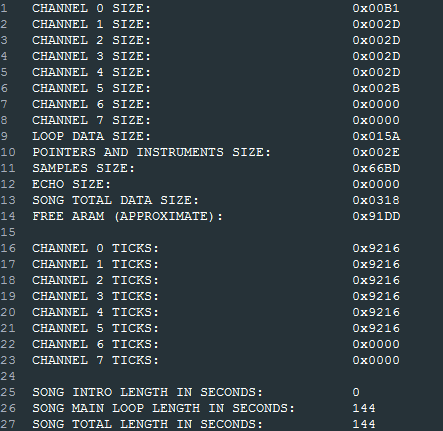
\includegraphics[width=.80\linewidth]{images/stats.png}
	\caption{Statistiken eines Songs}
	\label{stats}
\end{figure}

Channel Size 0 bis 7 geben die allgemeine Größe in Bytes als Hexwert dargestellt an,
Loop Data Size, wie viel Speicher durch das definieren der Loops selbst und deren Inhalte verbraucht wird und Pointers and Instruments Size von Pointern und Instrumentendefinitionen. \\
Die Summe dieser Werte ergibt die Total Data Size (auch Insert Size genannt) die beispielsweise angegeben werden muss, wenn ein Song auf SMW Central hochgeladen werden soll. \\
Samples Size gibt die Größe aller eingebundenen Samples und der Samples aus der Sample Group an, Echo Size von Echo, falls man diesen aktiviert.

\bigskip

Wird die Summe aus Insert Size, Samples Size und Echo Size von 64kB abgezogen (die Menge an Arbeitsspeicher vom SPC700) erhalten wir den Free ARAM (approximate) Wert, also jener Wert, der den freien Speicher im Audio Ram angibt. \\
Von diesem Wert müssen wir aber ungefähr 0x2700 Bytes abziehen (ca. 10kB), sofern keine Global Songs oder Sample Groups geändert wurden. Dieser Platz wird von der Musik Engine, Soundeffekten und Global Songs dauerhaft eingenommen und wird nicht in der Rechnung im Stats Textdokument berücksichtigt. Wird beispielsweise ein Global Song ausgetauscht, ändert sich die Grenze entsprechend.

\bigskip

Channel Ticks 0 - 7 geben die Länge der Kanäle in Ticks an, wobei es sich hierbei um Dezimalzahlen und nicht um Hexwerte handelt, trotz des fälschlicherweise verwendeten Präfixes. Im Idealfall besitzen alle verwendeten Kanäle die gleiche Länge, da der kürzeste Kanal die Gesamtdauer des Songs angibt.

\bigskip

Die letzten 3 Werte geben die Länge des Intros, des geloopten Song selbst und der Summe aus Intro und geloopten Song in Sekunden an.

\subsection{Hexbefehle}

Hexbefehle sind einfach durch ihren Aufbau zu identifizieren. Sie beginnen mit einem \$ und einer Befehlsnummer als Hexadezimalzahl, gefolgt von ein bis maximal 3 Hexwerten (einzige Ausnahme sind die Filter Koeffizienten).
\bigskip

Falls ein Befehl eine Länge oder Dauer als Parameter verwendet, handelt es sich hierbei immer um einen Tick Wert im Hexadezimalsystem. Eine Tabelle für einige Standardlängen findet sich im Anhang in Tabelle \ref{tickshex}.

\subsubsection{Pan Fading}

Pan Fading beschreibt den Verlauf der Lautstärke eines Instruments zwischen den Lautsprechern.

\medskip

\lstinputlisting[framexleftmargin=8mm, frame=shadowbox, rulesepcolor=\color{blue}, numbers=left, firstline=2, lastline=2]{codes/Hex.txt}

\medskip

mit 

\begin{itemize}
	\item Dauer \$XX 
	\item Ziel Panning \$YY
\end{itemize}

wobei \$00 y0 (Lautstärke vollständig rechts), \$0A y10 (Lautstärke gleichmäßig verteilt) und \$14 y20 (Lautstärke vollständig links) entspricht.

\subsubsection{Tempo Fading}

Tempo Fading beschreibt den globalen Verlauf des Tempos.

\medskip

\lstinputlisting[framexleftmargin=8mm, frame=shadowbox, rulesepcolor=\color{blue}, numbers=left, firstline=4, lastline=4]{codes/Hex.txt}

\medskip

mit 

\begin{itemize}
	\item Dauer \$XX 
	\item Ziel Panning \$YY
\end{itemize}

Dabei kann sich der Befehl in einem beliebigen Kanal befinden.

\subsubsection{Global volume Fading}

Global Volume Fading beschreibt den Verlauf der globalen Lautstärke.

\medskip

\lstinputlisting[framexleftmargin=8mm, frame=shadowbox, rulesepcolor=\color{blue}, numbers=left, firstline=6, lastline=6]{codes/Hex.txt}

\medskip

mit

\begin{itemize}
	\item Dauer \$XX 
	\item Ziel Lautstärke \$YY
\end{itemize}

Dabei kann sich der Befehl in einem beliebigen Kanal befinden.

\subsubsection{Vol Fading}

Volume Fading beschreibt den Verlauf der Lautstärke eines einzelnen Kanals.

\medskip

\lstinputlisting[framexleftmargin=8mm, frame=shadowbox, rulesepcolor=\color{blue}, numbers=left, firstline=8, lastline=8]{codes/Hex.txt}

\medskip

mit 

\begin{itemize}
	\item Dauer \$XX
	\item Ziel Lautstärke \$YY 
\end{itemize}

\subsubsection{Pitch Bending}

Pitch Bending schreibt den Verlauf des Pitches einer Note. Prominentes Beispiel dafür ist eine Gitarrensaite, die man nach oben oder unten schiebt.

\medskip

\lstinputlisting[framexleftmargin=8mm, frame=shadowbox, rulesepcolor=\color{blue}, numbers=left, firstline=10, lastline=10]{codes/Hex.txt}

\medskip

mit

\begin{itemize}
	\item Verzögerung \$XX
	\item Dauer \$YY
	\item Ziel Note \$ZZ
\end{itemize}

Der Befehl steht hinter der Note, die ein Pitch Bending erfahren soll. \\
Die Verzögerung gibt an, wann der Befehl ausgeführt werden soll, die Dauer gibt an wie lange das Bending dauert. Der Hexwert \$ZZ, der eine Note beschreibt, ist in Tabelle \ref{Noten} nachzulesen.

\begin{table}
\begin{tabularx}{\textwidth}{|l|X|X|X|X|X|X|X|X|X|X|X|X|}
	\hline
	& C & C\# & D & D\# & E & F & F\# & G & G\# & A & A\# & B   \\
	\hline
	o1 & 80 & 81 & 82 & 83 & 84 & 85 & 86 & 87 & 88 & 89 & 8A & 8B \\
	\hline
	02 & 8C & 8D & 8E & 8F & 90 & 91 & 92 & 93 & 94 & 95 & 96 & 97 \\
	\hline
	o3 & 98 & 99 & 9A & 9B & 9C & 9D & 9E & 9F & A0 & A1 & A2 & A3 \\
	\hline
	o4 & A4 & A5 & A6 & A7 & A8 & A9 & AA & AB & AC & AD & AE & AF \\
	\hline
	o5 & B0 & B1 & B2 & B3 & B4 & B5 & B6 & B7 & B8 & B9 & BA & BB \\
	\hline
	o6 & BC & BD & BE & BF & C0 & C1 & C2 & C3 & C4 & C5 & & \\
	\hline
\end{tabularx}
\caption{Noten als Hexwerte}
\label{Noten}
\end{table}


Es gibt zudem Wege, den Befehl einfacher auszuführen.

\bigskip

Anstelle des \$ZZ Wertes kann auch direkt eine Note angegeben werden (inklusive Oktavwechsel). Wichtigster Unterschied ist, dass durch ein Pitch Bending mit \$ZZ kein Oktavwechsel für nachfolgende Noten statt findet. Beispiel:

\medskip

\lstinputlisting[framexleftmargin=8mm, frame=shadowbox, rulesepcolor=\color{blue}, numbers=left, firstline=11, lastline=12]{codes/Hex.txt}

\medskip

Beide Befehle führen ein Pitch Bending von o3f nach o4c durch, allerdings ist die nachfolgende Note im ersten Befehl ein o3e und im zweiten ein o4e.

\bigskip

Zusätzlich kann durch den Einsatz von Haltebögen ein Hexbefehl anschaulicher beschrieben werden, in einigen Fällen sind diese auch notwendig um innerhalb einer Note mehrere oder unterschiedliche Befehle auszuführen. Beispiel:

\medskip

\lstinputlisting[framexleftmargin=8mm, frame=shadowbox, rulesepcolor=\color{blue}, numbers=left, firstline=13, lastline=14]{codes/Hex.txt}

\medskip

Beide Befehle beschreiben den gleichen Vorgang. Der erste Befehl wird erst nach der Verzögerungszeit von \$30 Ticks (entspricht der Länge einer Viertelpause) ausgeführt. Der zweite Befehl spielt die c+4 Note, ohne den Pitch Bending Befehl zu benutzen, der Befehl wird dann aber auf den Teil des Haltebogens sofort angewendet. Dieses Beispiel verdeutlicht auch, dass Vorsicht geboten ist bei Noten mit Haltebögen, die mit Pitch Bendings bearbeitet werden sollen.

\bigskip

Außerdem muss darauf geachtet werden, Haltebögen bei Noten mit Notenlängen größer 2 richtig anzuwenden. AddMusicK interpretiert diese intern auch mit Haltebögen. Ein c1 wird von AddMusicK beispielsweise als ein c2\textasciicircum2 gehandhabt. Dadurch entstehen Fehler. Beispiel:

\medskip

\lstinputlisting[framexleftmargin=8mm, frame=shadowbox, rulesepcolor=\color{blue}, numbers=left, firstline=15, lastline=16]{codes/Hex.txt}

\medskip

Zeile 2 zeigt, wie der Befehl der ersten Zeile von AddMusicK interpretiert wird. Das Pitch Bending würde nie ausgeführt werden, da eine halbe Note lang nichts passiert und danach eine weitere halbe Note lang (\$60) Verzögert wird, bis der Befehl ausgeführt werden soll. Es wird also eine ganze Note lang gewartet, bevor überhaupt das Bending beginnen würde.

Soll c1 nach einer halben Note das Pitch Bending beginnen, muss der Befehl wie folgt umgeschrieben werden:

\medskip

\lstinputlisting[framexleftmargin=8mm, frame=shadowbox, rulesepcolor=\color{blue}, numbers=left, firstline=17, lastline=17]{codes/Hex.txt}

\medskip



\subsubsection{Vibrato}

Vibrato beschreibt das Schwingen um eine Tonhöhe.

\medskip

\lstinputlisting[framexleftmargin=8mm, frame=shadowbox, rulesepcolor=\color{blue}, numbers=left, firstline=19, lastline=19]{codes/Hex.txt}

\medskip

mit

\begin{itemize}
	\item Verzögerung \$XX
	\item Frequenz  \$YY, wie schnell geschwungen wird
	\item Amplitude \$ZZ, mit der um eine Note geschwungen wird
\end{itemize}

Der Befehl wird auf alle nachfolgenden Noten des Kanals angewendet. \\
Mit \$DF kann das Vibrato ausgeschaltet werden. \\
Zusätzlich kann Vibrato Fading eingestellt werden:

\medskip

\lstinputlisting[framexleftmargin=8mm, frame=shadowbox, rulesepcolor=\color{blue}, numbers=left, firstline=20, lastline=20]{codes/Hex.txt}

\medskip

mit

\begin{itemize}
	\item Dauer \$XX
\end{itemize}

Dabei muss Vibrato Fading immer nach Vibrato benutzt werden, da sich der \$EA Befehl auf die \$YY und \$ZZ Werte von \$DE bezieht. Beispiel:

\medskip

\lstinputlisting[framexleftmargin=8mm, frame=shadowbox, rulesepcolor=\color{blue}, numbers=left, firstline=21, lastline=22]{codes/Hex.txt}

\medskip

Die erste Zeile beschreibt ein c1, dass nach der Dauer einer halben Note anfängt zu schwingen.
Die zweite Zeile beschreibt ein c1, dass nach der Dauer einer halben Note anfängt, anzuschwingen,
und erreicht das vorher definierte Vibrato Verhalten nach einer Viertelnote.


\subsubsection{ADSR / Gain einstellen}

ADSR kann während der Laufzeit verändert werden.

\medskip

\lstinputlisting[framexleftmargin=8mm, frame=shadowbox, rulesepcolor=\color{blue}, numbers=left, firstline=24, lastline=24]{codes/Hex.txt}

\medskip

wobei der Da Wert zwischen \$00 und \$7F liegen muss, ansonsten wird Gain aktiviert.

\bigskip

Genauso kann Gain umgestellt werden.

\medskip

\lstinputlisting[framexleftmargin=8mm, frame=shadowbox, rulesepcolor=\color{blue}, numbers=left, firstline=25, lastline=25]{codes/Hex.txt}

\medskip

mit \$YY dem Gain Wert. \$80 kann auch größer sein, darf aber nicht kleiner sein, ansonsten wird ADSR aktiviert. \\

Wird ein Instrument mit @ aufgerufen, werden die ADSR bzw. Gain Werte, die durch \$ED eingestellt wurden, zurückgesetzt. \\
Weitere Informationen zu ADSR und Gain siehe Kapitel \ref{sec:ADSR} und \ref{sec:Gain}.

\subsubsection{Echo}

Mit Echo kann der Raumklang eingestellt werden.

\medskip

\lstinputlisting[framexleftmargin=8mm, frame=shadowbox, rulesepcolor=\color{blue}, numbers=left, firstline=27, lastline=27]{codes/Hex.txt}

\medskip

mit

\begin{itemize}
	\item Kanäle \$XX
	\item Echo Lautstärke links \$YY
	\item Echo Lautstärke rechts \$ZZ
\end{itemize}

Welche Kanäle Echo erfahren sollen, wird mit \$XX festgelegt. Diese werden Bitweise durch die Kanäle in umgekehrter Reihenfolge bestimmt und letztendlich als Hexwert dargestellt. Ein Beispiel:

\bigskip

Die Kanäle 5, 6 und 7 (\#4, \#5 und \#6) sollen Echo erhalten. Wir schreiben die Kanalnummern absteigend auf und setzen eine 1 für Echo, ansonsten 0.

\begin{table}[htbp]
	\centering
	\begin{tabularx}{8.5cm}{|X|c|c|c|c|c|c|c|c|}
		\hline
		Kanalnummer: & 7 & 6 & 5 & 4 & 3 & 2 & 1 & 0 \\
		\hline
		Bits: & 0 & 1 & 1 & 1 & 0 & 0 & 0 & 0 \\
		\hline
	\end{tabularx}
\end{table}


Wir erhalten die Binärzahl 0b1110000 (0b ist der Präfix für Binärzahlen). Als Hexadezimalzahl ist dies \$70.

\bigskip

Zusätzlich müssen weitere Parameter eingestellt werden, um Echo zu aktivieren.

\medskip

\lstinputlisting[framexleftmargin=8mm, frame=shadowbox, rulesepcolor=\color{blue}, numbers=left, firstline=28, lastline=28]{codes/Hex.txt}

\medskip

mit

\begin{itemize}
	\item Echo Verzögerung \$XX
	\item Reverberation \$YY
	\item FIR Filter \$ZZ
\end{itemize}

Beide Befehle treten immer zusammen auf. \\

\$XX muss zwischen \$01 und \$0F liegen, bei \$00 ist Echo deaktiviert. Hierbei ist aber aufzupassen, da der Echo Delay Wert maßgeblich den Ram Speicher beeinträchtigt. Die Echo Size kann berechnet werden, indem man den \$XX Wert mit 2kB multipliziert. \$0F Echo Delay nimmt also 30kB Platz ein, was knapp die Hälfte des gesamten Audio RAMs entspricht.

\bigskip

Reverberation (kurz Reverb, deutsch: Nachhall) beschreibt die kontinuierliche Reflexion von Schallwellen in einem geschlossenen Raum, die sich im Vergleich zum Direktschall durch lange Laufzeiten auszeichnet. Durch Reverb lässt sich der Hall eines Raumes simulieren, zwei extreme wären beispielweise eine Kirche (großer Hall) und ein Tonstudio (kein Hall).

\bigskip

\$ZZ kann entweder auf \$01 (an) bzw. \$00 (aus) gestellt werden. Voreingestellt ist das FIR Filter (Finite Impulse Response, deutsch: Endliche Impulsantwort) beschrieben mit dem 1. Filterkoeffizienten auf \$7F und alle weiteren auf \$00. \\
Es ist auch möglich seinen eigenen FIR Filter zu designen mit dem folgenden Befehl:

\medskip

\lstinputlisting[framexleftmargin=8mm, frame=shadowbox, rulesepcolor=\color{blue}, numbers=left, firstline=29, lastline=29]{codes/Hex.txt}

\medskip

Hierdurch lassen sich verschiedene Filterformen realisieren, beispielsweise, Hochpass- oder Tiefpassfilter.
Das Filter lässt sich nur auf das Echo Signal anwenden.

\bigskip

Mit \$F4 \$03 kann Echo in einem Kanal umgeschaltet werden. Dies ist notwendig, falls ein Kanal verschiedene Instrumente verwendet, auf die nicht alle Echo angewandt werden soll.

\subsubsection{Yoshi Drums}

Falls ein Song den Yoshi Drums Befehl verwendet, ist der 5. Kanal (\#4) so lange stumm, bis Mario sich auf Yoshi setzt. Dabei kann sich alles mögliche in diesem Kanal befinden, der Befehl aktiviert Yoshi lediglich zu einem Schalter für den 5. Kanal.
\medskip

\lstinputlisting[framexleftmargin=8mm, frame=shadowbox, rulesepcolor=\color{blue}, numbers=left, firstline=31, lastline=31]{codes/Hex.txt}

\medskip



\subsubsection{Tremolo}
\subsubsection{Legato}
\subsubsection{Light Staccato}